
\section{Diseño}

\subsection{Especificaciones del circuito}
\bigskip
Se plantea un circuito con las siguientes características
\begin{itemize}
    \item \( f_o = 14 \, \) MHz
    \item \( Q_c = 10 \) 
    \item \( R_a = 50 \) $\Omega$
    \item \( R_L = 1 \) K$\Omega$ 
\end{itemize}

\subsection{Diseño del inductor}
Para el diseño de la bobina se realizó una tabla en Excel, donde se utilizó la siguiente ecuación:

\begin{equation}
    L = D^3 N_s^2 k \times 10^{-3} \, \mu \text{Hy}
\end{equation}

Donde:
\begin{itemize}
    \item \( D\, \) es el diámetro externo de la bobina, su unidad es en centímetros.
    \item \( N_s \) es el numero de espiras por unidad de longitud, su unidad es vueltas por centímetro.
    \item \( k\) es el factor de Nagaoka.
\end{itemize}
Con la ecuación (11) obtenemos el valor de la inductancia de la bobina. También debemos recordar otras variables que están implícitas dentro de la misma.
\begin{equation}
    N_s = \frac{N}{\ell} = \frac{1}{p} = \frac{1}{S_e+d}
\end{equation}
Donde:
\begin{itemize}
    \item \( N\, \) es el número de espiras, en vueltas.
    \item \( \ell\, \) es la longitud del inductor, en centímetros.
    \item \( p\, \) es el paso, en centímetros.
    \item \( S_e \) es la separación entre espiras, en centímetros. 
    \item \( d\) es el diámetro del conductor, en centímetros.
\end{itemize}

Para comenzar, se deben fijar algunos de estos parámetros. Se definen los siguientes:
\begin{itemize}
    \item \( D = 2 \, \) cm 
    \item \( d = 0,1 \, \) cm 
    \item \( S_e = 0,1 \) cm
\item \( \ell = 3 \) cm
\end{itemize}
Con esto, podemos calcular el factor de Nagaoka a través de las curvas, ingresando con \(\frac{\ell}{D}=1,5\) el cual resulta aproximadamente en \(k = 11,5\).
\newpage
\begin{figure}[!h]
    \centering
    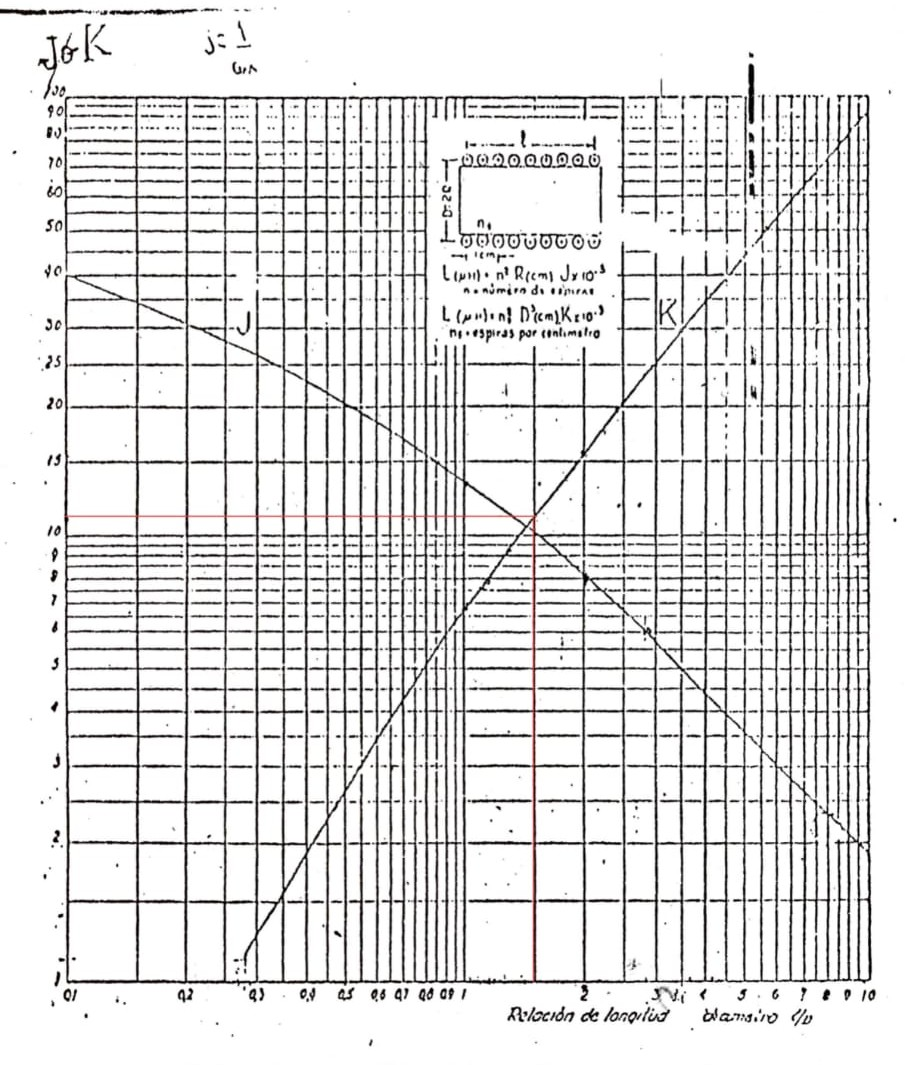
\includegraphics[scale=0.2]{Imagenes/CURVAK.jpeg}
    \caption{Curva K}
    \label{fig:K}
\end{figure}

Se calculan las variables faltantes:

\begin{equation}
    N_s =\frac{1}{0,1cm+0,1cm} = 5 \,\ \frac{v}{cm}
\end{equation}
Si bien \(N_s\) se requiere para calcular el valor del inductor, también se necesita saber cuantas vueltas tiene este para su construcción:
\begin{equation}
    N = N_s \ell = 5\frac{v}{cm}\times3cm = 15 \,\ vueltas
\end{equation}
Finalmente, se calcula la inductancia \(L\) mediante la ecuación (11):
\begin{equation}
    L = 2^3 \times 5^2 \times 11,5 \times 10^{-3} = 2,3\,\ \mu \text{Hy}
\end{equation}

\subsection{Cálculo de \(R_p\) y \(R_T\) }

Si se observa la ecuación (2), falta una variable de calcular para poder despejar \(R_p\). Dicha variable es \(Q_d\), la cual se calcula de la siguiente forma:
\begin{equation}
    Q_d = 8850\frac{D\ell}{102\ell+45D}\sqrt{f_o} = 8850\frac{2\cdot3}{102\cdot3+45\cdot2}\sqrt{14} = 501,72
\end{equation}
Luego, se despeja la ecuación (2) para obtener  \(R_p\):

\begin{equation}
    R_p = Q_dX_L = 501,72 \cdot 2\pi \cdot14\cdot 2,3 \cdot 10^{-6} = 101507,72 \Omega
\end{equation}


La resistencia \(R_T\) se despeja de la ecuación (3) sabiendo que \(BW = 1,4MHz\):
\begin{equation}
    R_T = \frac{f_o}{BW}X_L = \frac{14}{1,4}\cdot2\pi \cdot14\cdot 2,3 = 2023,19 \Omega
\end{equation}
\newpage
\subsection{Cálculo de \(R_a'\) y \(R_L'\)}
Para calcular \(R_a'\), se utiliza la ecuación (9):
\begin{equation}
    R_a' = 2\cdot R_T = 2 \cdot 2023,19\Omega = 4046,38 \Omega
\end{equation}
De igual manera con \(R_L'\) se utiliza la ecuación (8):
\begin{equation}
    R_L' = \frac{2\cdot R_TR_p}{R_p-2R_T} =  \frac{2\cdot 2023,19 \cdot 101507,72}{101507,72-2\cdot 2023,19} = 4214,37 \Omega
\end{equation}

\subsection{Cálculo de Capacitores}
Para el calculo de los capacitores, en primer lugar, se debe determinar la capacidad total \(C_T\), la cual se calcula mediante la ecuación (1):
\begin{equation}
    C_T = (\frac{1}{2\pi f_o\sqrt{L}})^2 = (\frac{1}{2\pi\cdot 14\cdot10^6\sqrt{2,3\cdot10^-6}})^2 = 56,19 \,\ pF
\end{equation}

Lo siguiente, es calcular los capacitores \(C_1, C_2, C_3 y C_4 \). Para ello se utilizarán las ecuaciones (5) y (6) para despejar los valores de dichos capacitores.
\begin{equation}
    C_2 = \frac{C_T}{2}\sqrt{\frac{R_a'}{R_a}} = \frac{C_T}{2}\sqrt{\frac{2R_T}{R_a}} = \frac{56,19pF}{2}\sqrt{\frac{2\cdot2023,19\Omega}{50\Omega}} = 272,74 \,\ pF
\end{equation}

\begin{equation}
    C_1 = \frac{C_2}{\sqrt{\frac{R_a'}{R_a}-1}} = \frac{272,74pF}{\sqrt{\frac{4046,38\Omega}{50\Omega}-1}} = 31,6 \,\ pF
\end{equation}

\begin{equation}
    C_4 = \frac{C_T}{2}\sqrt{\frac{R_L'}{R_L}} = \frac{C_T}{2}\sqrt{\frac{2R_TR_p}{R_L(R_p-2R_T)}} = \frac{56,19pF}{2}\sqrt{\frac{2\cdot2023,19\Omega \cdot 101507,72\Omega}{1000\Omega(101507,72\Omega-2\cdot2023,19\Omega)}} = 57,67 \,\ pF
\end{equation}

\begin{equation}
    C_3 = \frac{C_4}{\sqrt{\frac{R_L'}{R_L}-1}} = \frac{57,67pF}{\sqrt{\frac{4214,37\Omega}{1000\Omega}-1}} = 54,77 \,\ pF
\end{equation}




